\documentclass[dvipsnames,format=sigconf]{acmart}


\acmDOI{10.1145/nnnnnnn.nnnnnnn} % To be updated after completing copyright process
\acmISBN{978-x-xxxx-xxxx-x/YY/MM} % To be updated after completing copyright process
\acmConference[GECCO '24]{The Genetic and Evolutionary Computation Conference 2024}{July 14--18, 2024}{Melbourne, Australia}
\acmYear{2024}
\copyrightyear{2024}

%%
%% Submission ID.
%% Use this when submitting an article to a sponsored event. You'll
%% receive a unique submission ID from the organizers
%% of the event, and this ID should be used as the parameter to this command.
%%\acmSubmissionID{123-A56-BU3}

%%
%% For managing citations, it is recommended to use bibliography
%% files in BibTeX format.
%%
%% You can then either use BibTeX with the ACM-Reference-Format style,
%% or BibLaTeX with the acmnumeric or acmauthoryear sytles, that include
%% support for advanced citation of software artefact from the
%% biblatex-software package, also separately available on CTAN.
%%
%% Look at the sample-*-biblatex.tex files for templates showcasing
%% the biblatex styles.
%%

%%
%% The majority of ACM publications use numbered citations and
%% references.  The command \citestyle{authoryear} switches to the
%% "author year" style.
%%
%% If you are preparing content for an event
%% sponsored by ACM SIGGRAPH, you must use the "author year" style of
%% citations and references.
%% Uncommenting
%% the next command will enable that style.
%%\citestyle{acmauthoryear}


\usepackage{adjustbox}
\usepackage{algorithmic}
\usepackage{amsmath,amsfonts}
% \usepackage{array}
% \usepackage{authblk}
% \usepackage{bibunits}
% \usepackage{booktabs}
\usepackage{caption}
\usepackage{cite}
% \usepackage{colortbl}
\usepackage{csvsimple}
% \usepackage{csquotes}
% \usepackage{etoolbox}
\usepackage{graphicx}
\usepackage{hyperref,cleveref}
% \usepackage{import}
% \usepackage{natbib}[sort]
% \usepackage{rotating}
% \usepackage[subtle]{savetrees}
\usepackage{siunitx}
\usepackage{subcaption}
\usepackage{tabularx}
\usepackage{textcomp}
\usepackage{xcolor}
% \usepackage{lib/alifeconf}
\usepackage{orcidlink}
% \usepackage{pdflscape,longtable}
% \usepackage{listings}
% \usepackage{placeins}
\usepackage{pythonhighlight}

\IEEEoverridecommandlockouts
\IEEEaftertitletext{\vspace{-3\baselineskip}}

\input{lib/pragmaonce.tex}

\ifdefined\mydraft
\mydraft
\fi

\begin{document}

\title{ Trackable Agent-based Evolution Models at Wafer Scale}

\author[1]{Anonymized for Review}
% \author[1,2,3,*]{Matthew Andres Moreno\orcidlink{0000-0003-4726-4479}}
% \author[4]{Connor Yang\orcidlink{0009-0004-1240-2362}}
% \author[5,6]{Emily Dolson\orcidlink{0000-0001-8616-4898}}
% \author[1,2]{Luis Zaman\orcidlink{0000-0001-6838-7385}}

\affil[1]{Anonymized for Review}

% \affil[.  ]{\vspace{-4.4ex}}
% \affil[1]{Department of Ecology and Evolutionary Biology, University of Michigan, Ann Arbor, United States}
% \affil[2]{Center for the Study of Complex Systems, University of Michigan, Ann Arbor, United States}
% \affil[3]{Michigan Institute for Data Science, University of Michigan, Ann Arbor, United States}
% \affil[4]{Undergraduate Research Opportunities Program, University of Michigan, Ann Arbor, United States}
% \affil[5]{Department of Computer Science and Engineering, Michigan State University, East Lansing, United States}
% \affil[6]{Program in Ecology, Evolution, and Behavior, Michigan State University, East Lansing, United States}
% \affil[*]{corresponding author: \textit{morenoma@umich.edu}}

\maketitle


% \begin{bibunit}

\begin{abstract}
\vspace{-2ex}
% Continuing improvements in computing hardware are poised to transform capabilities for \textit{in silico} modeling of cross-scale phenomena underlying major open questions in evolutionary biology and artificial life, such as transitions in individuality, eco-evolutionary dynamics, and rare evolutionary events.
Emerging ML/AI-oriented hardware accelerators, like the 850,000 processor Cerebras Wafer Scale Engine (WSE), hold great promise to scale up the capabilities of evolutionary computation.
However, challenges remain in maintaining the telemetry necessary to assess the mode and tempo of evolution while efficiently utilizing these platforms' large processor counts.
Here, we focus on the problem of extracting phylogenetic information from agent-based evolution on the WSE platform.
% This goal drove significant refinements to decentralized \textit{in silico} phylogenetic tracking, reported here.
% These improvements yield order-of-magnitude performance improvements.
We present a tracking-enabled asynchronous island-based genetic algorithm (GA) framework for WSE hardware.
Emulated and on-hardware GA benchmarks with a simple tracking-enabled agent model clock upwards of 1 million generations a minute for population sizes reaching 16 million.
This pace enables quadrillions of evaluations a day.
We validate phylogenetic reconstructions from these trials and demonstrate their suitability for inference of underlying evolutionary conditions.
In particular, we demonstrate extraction, from wafer-scale simulation, of clear phylometric signals that differentiate runs with adaptive dynamics enabled versus disabled.
Together, these benchmark and validation trials reflect strong potential for highly scalable evolutionary computation that is both efficient and observable.
% Developed capabilities will bring entirely new classes of previously intractable research questions within reach, benefiting further explorations within the evolutionary biology and artificial life communities across a variety of emerging high-performance computing platforms.
\end{abstract}


\section{Introduction} \label{sec:introduction}

example \citep{gagliardi2019international}


\section{Methods} \label{sec:methods}

In this section, we describe the primary two algorithmic components for our on-device simulation:
\begin{enumerate}
\item the lightweight hereditary stratigraphy element used to annotate virtual genomes and facilitate robust post-hoc phylogenetic reconstruction, and
\item the asynchronous compute-communicate cycle used to instantiate an island model evolutionary process across the WSE engine.
\end{enumerate}


\begin{figure*}
  \centering
  \begin{subfigure}[t]{0.43\linewidth}
    \centering
  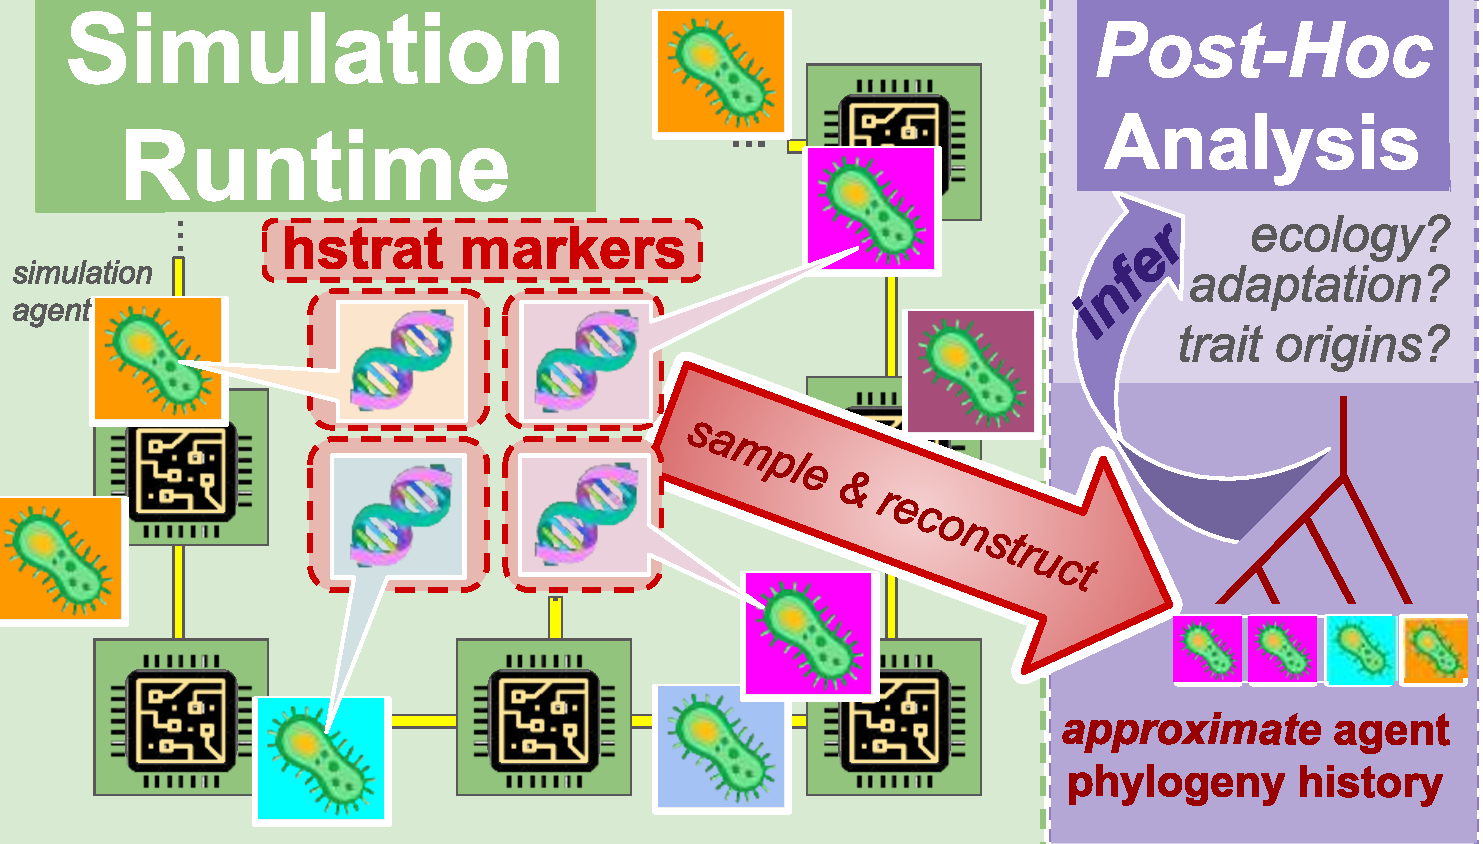
\includegraphics[width=\linewidth]{binder-wse-sketches/tex-access-proposal/img/runtime-posthoc-schematic}
    \caption{\footnotesize %
    hstrat markers help reconstruct phylogenies, which can tell evolutionary dynamics.
    }
    \label{fig:runtime-posthoc-schematic}
  \end{subfigure}
  \hspace{0.07\linewidth}
  \begin{subfigure}[t]{0.43\linewidth}
    \centering
  \includegraphics[width=\linewidth]{binder-wse-sketches/tex-access-proposal/img/async-ga-schematic}
    \caption{\footnotesize WSE island model evolutionary algorithm implementation.}
    \label{fig:async-ga-schematic}
  \end{subfigure}

\caption{%
\textbf{Methods for trackable distributed evolution simulation.}
\footnotesize
Subfigure \ref{fig:runtime-posthoc-schematic} shows use of hstrat markers to for reconstruct-based phylogenetic tracking of highly-distributed evolution simulations.
Subfigure \ref{fig:async-ga-schematic} summarizes asynchronous, callback-based approach to population exchange (``migration''') used to instantiate evolving populations across WSE PEs.
}
\label{fig:schematic}

\end{figure*}


\subsection{Distributed Phylogenetic Tracking}

Our approach to analysis of evolutionary history for wafer-scale simulation draws inspiration from the inference-based paradigm used to characterize history in natural systems.
This approach is fully-distributed, with ancestry information contained within genomes themselves rather than in any external tracking mechanism.
Just as mutational drift encodes ancestry information in DNA genomes, the inference-based paradigm requires only local updates to individual genomes at runtime as generations elapse.

Recent work introducing \textit{hereditary stratigraphy} (HStrat) methodology has explored how best to organize genetic material to maximize reconstruction quality and minimize memory footprint \citep{moreno2022hstrat, moreno2022hereditary}.
Proposed work bundles HStrat material with underlying agent genomes as an instrumentative ornament akin to non-coding DNA, entirely neutral with respect to agent traits or fitness.
Agents' \textit{HStrat} annotations can then be used to estimate their phylogenetic history after-the-fact, as depicted in Figure \ref{fig:runtime-posthoc-schematic}.

The hereditary stratigraphy algorithm associates each generation along individual lineages with an identifying ``fingerprint'' value, referred to as a differentia.
Each time a generation elapses, all offspring generate a new identifier value.
Within each offspring, generated identifiers append to an inherited running chronological record of differentia values.
To prevent $\mathcal{O}(n)$ space complexity as generations elapse, not all fingerprints can be kept.
Instead, excess fingerprints are pruned away according to a deterministic programme that ensures retention of differentia values from checkpoint generations spaced across evolutionary history.

Reducing differentia size also constitutes another important way to save memory space.
For instance, using a single-bit differentia would accrue a 32-fold savings over a one-word differentia and an 8-fold savings over a byte.
Although shrinking differentia size increases the probability of spurious collisions that result in overestimation of phylogenetic relatedness, this can be balanced by increasing the density with which differentiaare retained.
We anticipate that most scenarios will call for differentia sized on the order of a single bit or a byte.
However, benefits of small differentia cannot be accrued if differentia timepoints need to be stored.
In fact, storing one 32 or 64bit timestamp per differentia would likely bloat the majority of memory use for annotations, significantly reducing the amount of meaningful lineage-identifying differentia that can be stored.
Thus, existing algorithms provide calculations capabable of predicting the set of differentia that will be retained at any single point in time, allowing for the time stamps of differentia to be deduced solely from the current time point and the position of the site within the annotation.

Single-bit checkpoints have been shown to produce good quality phylogenies using only 96 bits per genome \citep{moreno2023toward}.
The semantic structure of HStrat annotations streamlines \textit{post hoc} phylogenetic reconstruction, which essentially boils down to a simple trie-building procedure
\citep{moreno2024analysis}.

Another notable complication in design of hereditary stratigraphy algorithms is the difference between ``steady'' and ``tilted'' retention patterns \citep{TODOFROMPREPRINT}.
In prior work, these are termed depth-proportional resolution and recency-proportional resolution.
This refers to the difffference in how retained time points are distributed over historical time.
For steady,retention, sampled time points are distributed evenly over history.
For tilted retention, more-recent time points are preferred.
So, there is tighter spacing between more recent time points and looser spacing between more ancient time points.
Intuitively, this reflects what is often the case in natural history work wehere we have higher absolute precision in pinpointing more recent events and looser absolute precision in pinpointing more ancient events.
Comparisons of reconstruction quality have shown that tilted algorithms give higher quality reconstructions for the same amount of space.
However, this is not always the case and new work (cite other paper) suggests that a hybrid approach where half of annotation space is allocated for each strategy may be robust and perform well across scenarios.
Figure \ref{fig:surf-algorithms} includes retention drip plots that illustrate the difference between steady and tilted algorithms.

\subsection{New Surface Algorithms}

Although designed with efficiency in mind, existing ``column''-based hereditary stratigraphy algorithms have several properties that make them a poor fit with a resource-constrained environment like the the Cerebras WSE:
\begin{enumerate}
\item an annotation size cap is guaranteed, but the entire space is not guaranteed to be used leading to a percentage of wasted space for strictly fixed-sized annotations,
\item current algorithm implementations use complex data structures with dynamically allocated memory to perform operations like set subtraction,
\item computation of retention policies can take time proportional to annotation size, with operations to maintain differentia in sorted order within the annotation also scaling linearly with annotation size, and
\item algorithms make use of divide and modulo operations, which are slow.
\end{enumerate}

\begin{figure}[b!]
  \centering
  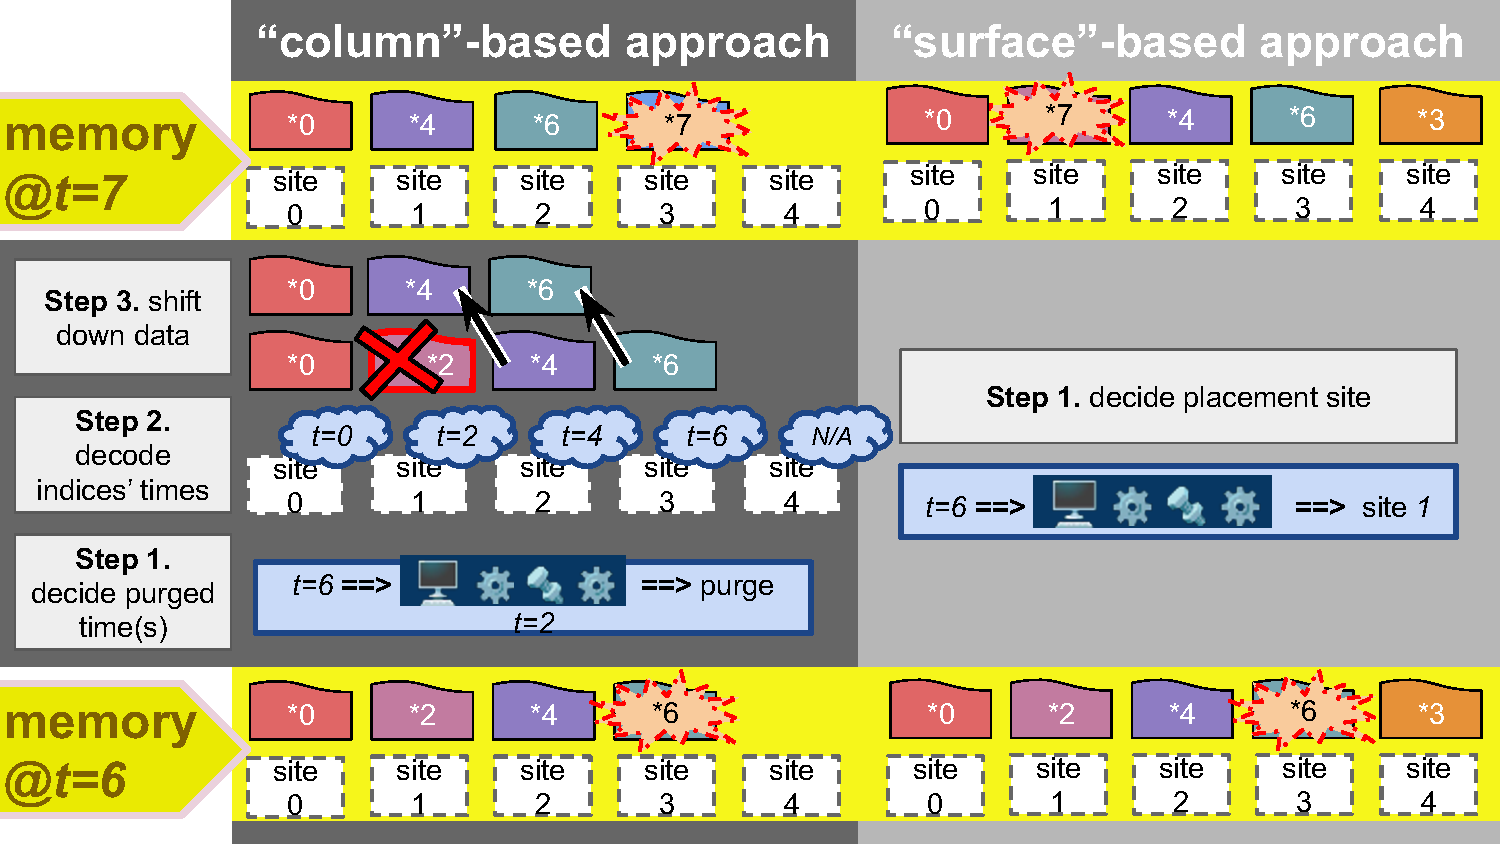
\includegraphics[width=0.95\linewidth]{img/surf-vs-column-schematic}

  \vspace{-1.5ex}

  \caption{
  \textbf{Column vs. surface-based hereditary stratigraphy.}
  \footnotesize
  Contrast of existing sorted-order ``column''-based stratum retention framework with proposed explicitly addressed ``surface''-based approach.}
  \label{fig:surf-vs-column-schematic}
  \vspace{-0.2in}
\end{figure}


Thus, the objectives of this project required significant elaboration of hereditary stratigraphy algorithms.
We use a constant-time indexing scheme that maps each lineage's fingerprint stream onto a fixed-width memory buffer such that eviction of existing fingerprint values by new placements maintains a temporally-representative sampling over elapsed time .
We call this approach ``surface''-based to distinguish it from earlier hereditary stratigraphy methods.
Time stamps can be positionally inferred and thus do not need to be stored --- a several-fold savings that enables fingerprint values to be shrunk down and packed together.
Figure \ref{fig:surf-vs=column-schematic} illustrates the difference between the existing ``column'' based approach and the new ``surface'' based approach which streamlines the annotation generational update procedure to a single operation.

\begin{figure*}
  \centering
\begin{subfigure}[b]{0.43\linewidth}
\centering
\textbf{steady retention policy}
\end{subfigure}
\begin{subfigure}[b]{0.43\linewidth}
\centering
\textbf{tilted retention policy}
\end{subfigure}

  \begin{subfigure}[b]{0.43\linewidth}
    \centering
  \includegraphics[height=\linewidth,angle=90,trim={0 2.4cm 0 0},clip]{binder-surface-concept/teeplots/10/cnorm=log+num-generations=4096+surface-size=256+viz=site-deposition-depth-by-rank-heatmap+ynorm=linear+ext=}
    \caption{256 bit steady surface site age plot}
    % \label{fig:runtime-posthoc-schematic}
  \end{subfigure}
  \begin{subfigure}[b]{0.43\linewidth}
    \centering
  \includegraphics[height=\linewidth,angle=90, trim={0 0 0 2.4cm},clip]{binder-surface-concept/teeplots/21/cnorm=log+num-generations=4096+surface-size=256+viz=site-deposition-depth-by-rank-heatmap+ynorm=linear+ext=}
    \caption{256 bit tilted surface site age plot}
    % \label{fig:async-ga-schematic}
  \end{subfigure}


\begin{subfigure}[b]{0.43\linewidth}
  \centering
\includegraphics[width=\linewidth,trim={0 0 0 0},clip]{binder-surface-concept/teeplots/10/num-generations=262144+surface-size=64+viz=stratum-persistence-dripplot+ext=}
  \caption{64 bit steady surface time retention plot}
  % \label{fig:runtime-posthoc-schematic}
\end{subfigure}
\begin{subfigure}[b]{0.43\linewidth}
  \centering
\includegraphics[width=\linewidth,trim={0 0 0 0},clip]{binder-surface-concept/teeplots/21/num-generations=262144+surface-size=64+viz=stratum-persistence-dripplot+ext=}
  \caption{64 bit tilted surface time retention plot}
  % \label{fig:async-ga-schematic}
\end{subfigure}

\caption{%
  Visualizations of steady (left) and tilted (right) surface site selection policies.
  Top row heatmaps shows evolution of time-since-last-deposition for each site on a 256 bit field over the course of 4,096 depositions.
  Bottom row drip plots show retention timelines for 3,000 ingested timepoints.
  Eliminated time points are marked in red.
  Note that for top row, time elapses from top to bottom.
  For bottom row, time elapses bottom to top.
  }
\label{fig:surf-algorithms}

\end{figure*}


Figure \ref{fig:surf-algorithms} depicts how our algorithms sequence depositions onto the surface (heatmap) and the resulting stratum retention patterns (drip plot).
We leave formal descriptions of the site selection algorithms developed for tilted and steady surface algorithms --- and the reverse procedure necessary to efficiently infer the deposition times of each site on a surface at an arbitrary timepoint in the surface to future work.
However, reference implementations of the described algorithms in Python are provided in supplementary material Listing TODO.
For this work, we also translated the tilted algorithm to Zig--like Cerebras Software Language for use on the WSE and, as an intermediate step, to the general-purpose Zig programming language.
These implementations can be found in associated software repositories with the project.

Notably, these algorithms are solving the more general problem of stream curation in a new and highly efficient way, and may find other uses in data stream applications \citep{TODOCITEPREPRINT}.

\subsection{Asynchronous Island-model Evolutionary Computation}

We apply an island-model genetic algorithm to instantiate an evolutionary process spanning PEs.
Island-model approaches are common in applications of parallel and distributed computing to evolutionary computation \citep{bennett1999building}.
Under this model, each processor element (PE) hosts an independent population.
Migration between PEs stitches island populations together into a common gene pool.

Core kernel activity proceeds via an update cycle performed on each PE, which comprises several steps.
Figure \ref{fig:async-ga-schematic} provides a schematic overview.

The first step of this update loop is to handle migration, depicted as blue-red arrows in Figure \ref{fig:async-ga-schematic}.
We adopt a fully asynchronous approach to migration between neighboring PEs.
Evolutionary processes tend to occur in asynchronous manner with arbitrary factors influencing things, so this is a reasonable relaxation to make.

Each PE maintains independent immigration buffers and emigration buffers dedicated to each cardinal neighbor, depicted in blue and red, respectively, in Figure \ref{fig:async-ga-schematic}.
On simulation startup, an asynchronous DSD receive operation is opened to accept genomes from neighboring PEs into the appropriate immigration buffer.
At startup, additionally, the emigration buffer is populated with one or more genomes copied the population.
Then, an asynchronous send request is opened to dispatch wavelets containing genome data from the emigration buffer to the neighbor.
Both operations register an on-completion callback to set a ``send complete'' or ``receive complete'' flag variable associated with their corresponding buffer.

Each update cycle, the main update loop tests all ``send complete'' and ``receive complete'' flags.
For each immigration flag that is set, corresponding received genomes are written into the main population buffer, replacing randomly-chosen population members.
Then, the flag is reset a new receive request is initiated.
Likewise, for each emigration flag set, corresponding send buffers are re-populated with randomly sampled genomes from the main population buffer.
Corresponding flags are then reset and new send requests initiated.
The bottom right corner of Figure \ref{fig:async-ga-schematic} summarizes this process.

The remainder of the main update loop handles evolutionary operations within the scope of the executing PE.
Each genome within the population is evaluated to produce a floating point fitness value.
Modular implementation ensures evaluation criteria can be chosen appropriate for underlying experimental objectives.
For the purposes this project, we will use a trivial fitness function that explicitly models additive accumulation of beneficial/deleterious mutations as a floating point value within each genome.

After evaluation, tournament selection is applied.
Each slot in the next generation is populated with a genome exhibiting maximal fitness among $n$ randomly sampled individuals, ties broken randomly.

Finally, a mutational operator is applied across all genomes in the next population.
As with evaluation criteria, modular implementation allows mutation operations to be defined based on experimental objectives.
Here, we use a simple Gaussian mutation on each genome's stored fitness value.
At this point, hereditary stratigraphy annotations --- discussed next --- are updated to reflect an elapsed generation.

The process then repeats, with self-activating wavelet dispatched to execute the next cycle of the main update loop.

% Define lighter colors
\definecolor{LighterBlue}{rgb}{0.84, 0.92, 0.95}
\definecolor{LighterSalmon}{rgb}{1.0, 0.81, 0.76}
\definecolor{LighterPastelGreenYellow}{rgb}{0.88, 0.96, 0.90}

% Define thick vertical lines for section dividers
\newcolumntype{q}{!{\color{white} \vrule width 2pt}}

\begin{figure*}
    \centering
\begin{tabular}{
c
>{\columncolor{LighterBlue}}c
>{\columncolor{LighterBlue}}c
>{\columncolor{LighterSalmon}}c
>{\columncolor{LighterSalmon}}c
q % Thick divider
>{\columncolor{LighterPastelGreenYellow}}c
>{\columncolor{LighterPastelGreenYellow}}c
>{\columncolor{LighterPastelGreenYellow}}c
>{\columncolor{LighterPastelGreenYellow}}c
q % Thick divider
>{\columncolor{LighterPastelGreenYellow}}c
>{\columncolor{LighterPastelGreenYellow}}c
>{\columncolor{LighterPastelGreenYellow}}c
>{\columncolor{LighterPastelGreenYellow}}c
}
& \multicolumn{4}{cq}{\cellcolor{white}Word 0} & \multicolumn{4}{cq}{\cellcolor{white}Word 1} & \multicolumn{4}{c}{\cellcolor{white}Word 2} \\
\cmidrule(l{1.5pt}r{1.5pt}){2-5}
\cmidrule(l{1.5pt}r{1.5pt}){6-9}
\cmidrule(l{1.5pt}r{1.5pt}){10-13}
Byte & {\cellcolor{white}0} & {\cellcolor{white}1} & {\cellcolor{white}2} & {\cellcolor{white}3} & {\cellcolor{white}4} & {\cellcolor{white}5} & {\cellcolor{white}6} & {\cellcolor{white}7} & {\cellcolor{white}8} & {\cellcolor{white}9} & {\cellcolor{white}10} & {\cellcolor{white}11} \\
\cmidrule(l{1.5pt}r{1.5pt}){2-2}
\cmidrule(l{1.5pt}r{1.5pt}){3-3}
\cmidrule(l{1.5pt}r{1.5pt}){4-4}
\cmidrule(l{1.5pt}r{1.5pt}){5-5}
\cmidrule(l{1.5pt}r{1.5pt}){6-6}
\cmidrule(l{1.5pt}r{1.5pt}){7-7}
\cmidrule(l{1.5pt}r{1.5pt}){8-8}
\cmidrule(l{1.5pt}r{1.5pt}){9-9}
\cmidrule(l{1.5pt}r{1.5pt}){10-10}
\cmidrule(l{1.5pt}r{1.5pt}){11-11}
\cmidrule(l{1.5pt}r{1.5pt}){12-12}
\cmidrule(l{1.5pt}r{1.5pt}){13-13}
& \multicolumn{4}{cq}{\cellcolor{white}} & \multicolumn{4}{cq}{\cellcolor{white}} & \multicolumn{4}{c}{\cellcolor{white}} \\[-2ex]
Genome 0 & \texttt{F9} & \texttt{02} & \texttt{79} & \texttt{00} & \texttt{8D} & \texttt{22} & \texttt{4F} & \texttt{F3} & \texttt{D2} & \texttt{78} & \texttt{AD} & \texttt{C7} \\
& \multicolumn{4}{cq}{\cellcolor{white}} & \multicolumn{4}{cq}{\cellcolor{white}} & \multicolumn{4}{c}{\cellcolor{white}} \\[-2ex]
Genome 1 & \texttt{F9} & \texttt{02} & \texttt{75} & \texttt{00} & \texttt{8D} & \texttt{A1} & \texttt{CB} & \texttt{F2} & \texttt{D1} & \texttt{5B} & \texttt{CC} & \texttt{D4} \\
& \multicolumn{4}{cq}{\cellcolor{white}} & \multicolumn{4}{cq}{\cellcolor{white}} & \multicolumn{4}{c}{\cellcolor{white}} \\[-2ex]
Genome 2 & \texttt{61} & \texttt{B6} & \texttt{65} & \texttt{00} & \texttt{66} & \texttt{29} & \texttt{B4} & \texttt{F0} & \texttt{62} & \texttt{99} & \texttt{5A} & \texttt{61} \\
{\cellcolor{white}\ldots} & {\cellcolor{white}\ldots} & {\cellcolor{white}\ldots} & {\cellcolor{white}\ldots} & {\cellcolor{white}\ldots} & {\cellcolor{white}\ldots} & {\cellcolor{white}\ldots} & {\cellcolor{white}\ldots} & {\cellcolor{white}\ldots} & {\cellcolor{white}\ldots} & {\cellcolor{white}\ldots} &
{\cellcolor{white}\ldots} & {\cellcolor{white}\ldots} \\
\end{tabular}

\caption{%
\textbf{Example genomes sampled after simulation completion.}
  In validation testing, genomes were composed of three 32-bit words.
  The first two bytes (blue) are fixed random markers generated at simulation start-up, indicating independent lineage originations.
  The next two bytes (salmon) are a generation counter.
  Bits within the final eight bytes are lineage checkpoint values to facilitate phylogenetic reconstruction, arranged according to a tilted hereditary stratigraphic algorithm.
  Note that this genome does not include any content affecting agent traits or fitness --- neutral selection was used for this validation experiment.
}
\label{fig:genome-layout}
\end{figure*}


Kernel source code implementing described procedures can be viewed at \url{https://hopth.ru/cl}.
Our implementation is defined modularity with respect to genome size, layout, mutational operator, and fitness evaluation criteria, allowing for direct re-use of produced software for follow-on evolution experiments on WSE hardware.
Figure \ref{fig:genome-layout} shows an example genome layout including hstrat instrumentation.


In preparation for proposed work, we joined the Cerebras SDK program \citep{selig2022cerebras} and assembled Cerebras Software Language (CSL) software implementations that will be necessary to conduct experiments with WSE hardware.
For the time being, we have used Cerebras' hardware emulator to test our software implementations.
This section reports a small-scale experiment performed to validate the core software functionality.
In addition to this integration test, software quality has also been verified through an associated unit test suite.

Genomes were fixed-length 3 word arrays represented using data type \texttt{u32}.
Figure \ref{fig:validation-example:genomes} details the content and layout of genomes, and provides example genome values yielded from simulation.
Notably, the first sixteen bits were used to tag clade geneses.
At the outset of simulation, founding population members were each assigned a randomized tag value.
This value was inherited without mutation over the course of simulation.
Thus, it can be used to identify end-state genomes that evolved from the same original ancestor.

The send buffers were sized to hold one genome and the receive buffers to hold 4 genomes.

% A key question will be the extent to which intentionally desynchronizing affects performance, stability, and computation quality.

\subsection{Software and Data Availability}

Software, configuration files, and executable notebooks for this work are available at \url{https://github.com/mmore500/hstrat-wafer-scale} TODO.
CSL Software can be found on at \url{https://github.com/mmore500/wse-sketches/tree/v0.1.0} \citep{moreno2024wse}.
Data and supplemental materials are available via the Open Science Framework \url{https://osf.io/bfm2z/} \citep{foster2017open}.

All hereditary stratigraph annotation, reference phylogeny generation, and phylogenetic reconstruction tools used in this work are published in the \texttt{hstrat} Python package \citep{moreno2022hstrat}.
This project uses data formats and tools associated with the ALife Data Standards project \citep{lalejini2019data} and benefited from many pieces of open-source scientific software \citep{sand2014tqdist,2020SciPy-NMeth,harris2020array,reback2020pandas,mckinney-proc-scipy-2010,sukumaran2010dendropy,cock2009biopython,dolson2024phylotrackpy,torchiano2016effsize,waskom2021seaborn,hunter2007matplotlib,moreno2024apc,moreno2023teeplot,torchiano2016effsize,moreno2024pecking,moreno2024joinem,moreno2024hsurf}.

The experiments in this use the Cerebras SDK to compile and test on a hardware simulator \citep{TODOCITE}.
Access to the SDK can be requested, currently free of charge, via their website.


\section{Results and Discussion} \label{sec:results}

Here, we report a series of benchmarks that evaluate the viability of our proposed approaches to harness the CS-2 accelerator for digital evolution simulations and extract phylogenetic records from said simulations.
First, we compare the performance characteristics of new surface-oriented hereditary stratigraphy methods against preceding column-based implementation to determine the extent to which they succeed in streamlining runtime operations.
Then, we benchmark phylogeny-tracked WSE genetic algorithm implementations.
To assess the runtime overhead of surface-based tracking, we compare against benchmarking results with phylogenetic tracking disabled.
Finally, we validate the credibility of the presented end-to-end annotation-to-reconstruction pipeline by reviewing clade structure and phylometric properties from emulated and on-hardware runs.

\subsection{Surface Algorithm Benchmark on Conventional CPU}

We performed microbenchmark experiments to test computational efficiency of new surface-based algorithms.
Trials measured the real-time speed of sequential generation updates on one annotation with capacity for 64 differentiae.
Benchmarks used both Python, for comparability with existing column algorithm implementations, and Zig, to assess performance under compiler optimization.
Figure \ref{fig:benchmarking} overviews results.

% https://github.com/mmore500/hstrat-surface-concept/blob/51d636d768d474fc5148b9fcaa199c1b7776e915/benchmark.ipynb
Python implementations of the surface tilted and steady algorithms both took around 4.2 microseconds per operation (standard errors [SE] 50ns and 66ns; $n=20$).
For context, this speed was about $4\times$ the measured time for a surface placement using a trivial calculation (SE 0.05; $n=20$).
As expected, column implementations of steady and tilted fared much worse, taking about $7\times$ and $34\times$ the execution time per operation compared to the surface operations.
In both cases, surface implementations significantly outperformed their column counterparts (Mann-Whitney U test, $\alpha = 0.05$).
% While Python is an interpreted language and the Python-implemented algorithms weren't specifically implemented to maximize performance and suffer an intrinsic performance penalty due to that, the algorithms were all on the same footing and
% We use the ``optimize''' flag to strip superfluous safety checks.

% https://github.com/mmore500/wse-sketches/blob/d42e9174025bc67fa669347611d1a82b9ea5843c/binder/benchmark.ipynb
Zig microbenchmarks clock tilted surface annotation updates at 230 ns per operation (SE 0.9ns; $n=20$).
For context, this time is a little more than twice that required for a main memory access in contemporary computing hardware \citep{markus2022memory}.
Our results measure the operation at $49\times$ the measured time for a trivial placement calculation (SE 0.03; $n=20$).
Zig steady implementation clocks 511 ns per operation (SE 4; $n=20$), $110\times$ trivial (SE 0.8ns; $n=20$).
Note that speedup of Zig implementations relative to Python reflects an intrinsic performance penalty due to interpreter overhead of Python evaluation.
However, comparisons among Python implementations and among Zig implementations are nonetheless informative because all are on equal footing in this regard.

% \footnote{Steady results are not included, due to a Zig implementation not yet being completed.}

Low-hanging speedups and optimizations exist to further improve the per-operation surface update performance achieved in practice.
Half of update operations on surfaces with single-bit differentiae can be skipped entirely, owing to 50\% probability that randomization fails to change a stored differentia value.
Further, simulations with synchronous or near-synchronous generations can cache calculated surface-placement indices, meaning they would only need to be computed once for an entire subpopulation.
Another possibility is to coarsen temporal resolution, only updating annotations at intervals every $n$th generation.

\subsection{Wafer-Scale Engine Island-model GA Benchmark}

Next, we used an emulator to characterize the expected performance of our island model genetic algorithm on WSE hardware and estimate the magnitude of simulation that might be achieved with on-device execution.
We used the emulator's per-PE clock cycle counters to measure the amount of real time elapsed over the course of a 40-generation-cycle simulation.
We tested using a $3\times3$ PE collective with the tagged 3-word genome and a per-PE population size of 32, applying a tilted hereditary stratigraphy every generation.
PEs completed a mean of 24,138 generation cycles per second (SEM 99; $n=9$).
As an indicator of inter-PE exchange throughput, each PE immigrated a mean of 118 genomes (SEM 11; $n=9$) over 40 elapsed generation cycles.

% https://osf.io/tf89g
What scale of simulation does this performance imply at full scale on CS-2 hardware?
Across eight on-device, tracking-enabled trials of 1 million generations (described in the following section), we measured a mean simulation rate of 17,688 generations per second for 562,500 PEs ($750\times750$ rectangle) with run times slightly below one minute.
Trials with 1,600 PEs ($40\times40$) performed similarly, completing 17,734 generations per second.

Multiplied out to a full day, 17,000 generations per second turnover would elapse around 1.5 billion generations.
With 32 individuals hosted per each of 850,000 PEs, the net population size would sit around 27 million at full CS-2 wafer scale.
(Note, though, that available on-chip memory could support thousands of our very simple agents per PE, raising the potential for a net population size on the order of a billion agents.)
% 24,000 * 850,000 * 60 * 60 * 24 * 32 ---> ?? quadrillion
A naive extrapolation estimates on the order of a quadrillion agent replications could be achieved hourly at full wafer scale for such a very simple model.
We look forward to conducting more thorough benchmarking and scaling experiments in future work.
%The barebones simplicity of the model should also be noted.

How fast is simulation without hstrat instrumentation?
We repeated our hardware-emulated benchmark with 32-bit genomes stripped of all instrumentation.
Under these conditions, PEs completed on average 47,175 generations per second (SEM 220; $n=9$) and immigrated 118 genomes (SEM 12; $n=9$).

These timings measure phylogeny tracking as approximately equivalent to that of the other aspects of simulation, combined.
Given the highly minimalistic nature of the agent model and selection process, this result is highly promising.
In actual use, most experiments will likely involve a much more sophisticated agent model, so relative overhead of tracking will be diminished.
Additionally, these results do not include caching and coarsening strategies discussed above, which would speed tracking up considerably.

% https://github.com/mmore500/wse-sketches-mirror/actions/runs/8590107511/job/23537207835
% from https://github.com/mmore500/wse-sketches-mirror/commit/3a1bf8e9f2820a38cb7387a7624a86361485174b
% ASYNC_GA_GENOME_FLAVOR genome_purifyingplus
% ASYNC_GA_GLOBAL_SEED 0
% ASYNC_GA_NCYCLE_AT_LEAST 40
% ASYNC_GA_MSEC_AT_LEAST 0
% ASYNC_GA_TSC_AT_LEAST 0
% INFO: Using SIF: /home/runner/cerebras/bin/cbcore_sdk-202311111408-10-4a54bce5.sif
% INFO: User's specified CSL_IMPORT_PATH=
% NOTE: CSL_IMPORT_PATH accepts colon separated list of paths generated by 'realpath <path>'
% INFO:    Environment variable SINGULARITYENV_CSL_SUPPRESS_SIMFAB_TRACE is set, but APPTAINERENV_CSL_SUPPRESS_SIMFAB_TRACE is preferred
% compile successful
% Updated 1 path from the index
% CS_PYTHON cs_python
% INFO: Using SIF: /home/runner/cerebras/bin/cbcore_sdk-202311111408-10-4a54bce5.sif
% INFO:    Environment variable SINGULARITYENV_CSL_SUPPRESS_SIMFAB_TRACE is set, but APPTAINERENV_CSL_SUPPRESS_SIMFAB_TRACE is preferred
% whoami ===============================================================
% [[0 3 6]
%  [1 4 7]
%  [2 5 8]]
% whereami x ===========================================================
% [[0 1 2]
%  [0 1 2]
%  [0 1 2]]
% whereami y ===========================================================
% [[0 0 0]
%  [1 1 1]
%  [2 2 2]]
% cycle counter =======================================================
% [[40 40 40]
%  [40 40 40]
%  [40 40 40]]
% recv counter N ========================================================
% [[ 1  1  1]
%  [ 9 13 11]
%  [15 12 12]]
% recv counter S ========================================================
% [[ 7  9  8]
%  [10 11  9]
%  [ 1  1  1]]
% recv counter E ========================================================
% [[12 11  1]
%  [12 13  1]
%  [ 9 13  1]]
% recv counter W ========================================================
% [[ 1 11  9]
%  [ 1  7  9]
%  [ 1 10 11]]
% recv counter sum =====================================================
% [21, 32, 19, 32, 44, 30, 26, 36, 25]
% np.mean(recvSum)=29.444444444444443 np.std(recvSum)=7.304657739508267 sps.sem(recvSum)=2.5825865109265465
% send counter N ========================================================
% [[ 0  0  0]
%  [24 32 34]
%  [40 46 34]]
% send counter S ========================================================
% [[38 50 46]
%  [58 50 48]
%  [ 0  0  0]]
% send counter E ========================================================
% [[44 32  0]
%  [24 32  0]
%  [40 46  0]]
% send counter W ========================================================
% [[ 0 50 46]
%  [ 0 50 48]
%  [ 0 36 48]]
% send counter sum =====================================================
% [82, 132, 92, 106, 164, 130, 80, 128, 82]
% np.mean(sendSum)=110.66666666666667 np.std(sendSum)=27.744869395579748 sps.sem(sendSum)=9.809292646374773
% tscControl values ====================================================
% [30064968187, 30064968187, 30064968187, 30064968187, 30064968187, 30064968187, 30064968187, 30064968187, 30064968187]
% tscStart values ======================================================
% [2220, 2222, 2731, 2731, 1716, 2738, 3241, 3243, 3237]
% tscEnd values ========================================================
% [1414233, 1414662, 1406657, 1388294, 1438771, 1433887, 1412082, 1403426, 1390454]
% tsc diffs ============================================================
% --------------------------------------------------------------- ticks
% [1412013, 1412440, 1403926, 1385563, 1437055, 1431149, 1408841, 1400183, 1387217]
% np.mean(tsc_ticks)=1408709.6666666667 np.std(tsc_ticks)=16415.157825754963 sps.sem(tsc_ticks)=5803.63470641938
% -------------------------------------------------------------- seconds
% [0.0016611917647058824, 0.0016616941176470588, 0.0016516776470588235, 0.0016300741176470588, 0.0016906529411764705, 0.0016837047058823528, 0.00165746, 0.0016472741176470588, 0.00163202]
% np.mean(tsc_sec)=0.0016573054901960784 np.std(tsc_sec)=1.9311950383241098e-05 sps.sem(tsc_sec)=6.827805536963963e-06
% ---------------------------------------------------- seconds per cycle
% [4.152979411764706e-05, 4.154235294117647e-05, 4.129194117647059e-05, 4.075185294117647e-05, 4.226632352941176e-05, 4.209261764705882e-05, 4.1436499999999995e-05, 4.1181852941176466e-05, 4.0800500000000003e-05]
% np.mean(tsc_cysec)=4.143263725490196e-05 np.std(tsc_cysec)=4.827987595810268e-07 sps.sem(tsc_cysec)=1.7069513842409884e-07
% ---------------------------------------------------------- cycle hertz
% [24079.09842189838, 24071.81897992127, 24217.800653310787, 24538.761499837972, 23659.498070707108, 23757.135001317125, 24133.312417795907, 24282.540210815303, 24509.50356000539]
% np.mean(tsc_cyhz)=24138.829868401026 np.std(tsc_cyhz)=280.43062795032466 sps.sem(tsc_cyhz)=99.14719933803819
% --------------------------------------------------------- ns per cycle
% [41529.79411764706, 41542.35294117647, 41291.94117647059, 40751.852941176476, 42266.32352941176, 42092.61764705882, 41436.49999999999, 41181.85294117647, 40800.5]
% np.mean(tsc_cyns)=41432.63725490196 np.std(tsc_cyns)=482.7987595810264 sps.sem(tsc_cyns)=170.6951384240987
% fitness =============================================================
% [[0.00316905 0.00565182 0.0022315 ]
%  [0.00687918 0.00742484 0.00589414]
%  [0.00582986 0.0057458  0.00379858]]


% https://github.com/mmore500/wse-sketches-mirror/actions/runs/8590107511/job/23537207835
% from https://github.com/mmore500/wse-sketches-mirror/commit/3a1bf8e9f2820a38cb7387a7624a86361485174b
% CSLC cslc
% ASYNC_GA_GENOME_FLAVOR genome_purifyingstripped
% ASYNC_GA_GLOBAL_SEED 0
% ASYNC_GA_NCYCLE_AT_LEAST 40
% ASYNC_GA_MSEC_AT_LEAST 0
% ASYNC_GA_TSC_AT_LEAST 0
% INFO: Using SIF: /home/runner/cerebras/bin/cbcore_sdk-202311111408-10-4a54bce5.sif
% INFO: User's specified CSL_IMPORT_PATH=
% NOTE: CSL_IMPORT_PATH accepts colon separated list of paths generated by 'realpath <path>'
% INFO:    Environment variable SINGULARITYENV_CSL_SUPPRESS_SIMFAB_TRACE is set, but APPTAINERENV_CSL_SUPPRESS_SIMFAB_TRACE is preferred
% compile successful
% Updated 1 path from the index
% CS_PYTHON cs_python
% INFO: Using SIF: /home/runner/cerebras/bin/cbcore_sdk-202311111408-10-4a54bce5.sif
% INFO:    Environment variable SINGULARITYENV_CSL_SUPPRESS_SIMFAB_TRACE is set, but APPTAINERENV_CSL_SUPPRESS_SIMFAB_TRACE is preferred
% whoami ===============================================================
% [[0 3 6]
%  [1 4 7]
%  [2 5 8]]
% whereami x ===========================================================
% [[0 1 2]
%  [0 1 2]
%  [0 1 2]]
% whereami y ===========================================================
% [[0 0 0]
%  [1 1 1]
%  [2 2 2]]
% cycle counter =======================================================
% [[40 40 40]
%  [40 40 40]
%  [40 40 40]]
% recv counter N ========================================================
% [[ 1  1  1]
%  [13 11 14]
%  [11  7 11]]
% recv counter S ========================================================
% [[ 9 13  9]
%  [11 13 11]
%  [ 1  1  1]]
% recv counter E ========================================================
% [[11 15  1]
%  [ 7 11  1]
%  [ 7  9  1]]
% recv counter W ========================================================
% [[ 1  7  9]
%  [ 1  9 13]
%  [ 1 11 13]]
% recv counter sum =====================================================
% [22, 36, 20, 32, 44, 39, 20, 28, 26]
% np.mean(recvSum)=29.666666666666668 np.std(recvSum)=8.16496580927726 sps.sem(recvSum)=2.886751345948129
% send counter N ========================================================
% [[ 0  0  0]
%  [38 52 38]
%  [42 52 44]]
% send counter S ========================================================
% [[54 44 56]
%  [44 30 44]
%  [ 0  0  0]]
% send counter E ========================================================
% [[28 38  0]
%  [38 52  0]
%  [42 52  0]]
% send counter W ========================================================
% [[ 0 44 56]
%  [ 0 30 44]
%  [ 0 30 38]]
% send counter sum =====================================================
% [82, 126, 112, 120, 164, 126, 84, 134, 82]
% np.mean(sendSum)=114.44444444444444 np.std(sendSum)=26.192073063391234 sps.sem(sendSum)=9.260296238228726
% tscControl values ====================================================
% [30064968187, 30064968187, 30064968187, 30064968187, 30064968187, 30064968187, 30064968187, 30064968187, 30064968187]
% tscStart values ======================================================
% [1131, 1130, 1644, 1641, 628, 1650, 2151, 2155, 2149]
% tscEnd values ========================================================
% [709983, 736796, 714836, 730020, 721384, 731436, 713213, 730922, 713242]
% tsc diffs ============================================================
% --------------------------------------------------------------- ticks
% [708852, 735666, 713192, 728379, 720756, 729786, 711062, 728767, 711093]
% np.mean(tsc_ticks)=720839.2222222222 np.std(tsc_ticks)=9500.522988853212 sps.sem(tsc_ticks)=3358.9421151183965
% -------------------------------------------------------------- seconds
% [0.0008339435294117647, 0.0008654894117647059, 0.0008390494117647059, 0.0008569164705882353, 0.0008479482352941177, 0.0008585717647058823, 0.0008365435294117647, 0.0008573729411764705, 0.00083658]
% np.mean(tsc_sec)=0.0008480461437908496 np.std(tsc_sec)=1.1177085869239065e-05 sps.sem(tsc_sec)=3.9516966060216395e-06
% ---------------------------------------------------- seconds per cycle
% [2.0848588235294117e-05, 2.1637235294117648e-05, 2.097623529411765e-05, 2.1422911764705883e-05, 2.119870588235294e-05, 2.1464294117647056e-05, 2.0913588235294118e-05, 2.1434323529411762e-05, 2.0914499999999998e-05]
% np.mean(tsc_cysec)=2.1201153594771243e-05 np.std(tsc_cysec)=2.7942714673097676e-07 sps.sem(tsc_cysec)=9.879241515054106e-08
% ---------------------------------------------------------- cycle hertz
% [47964.878423140515, 46216.62547949749, 47672.99689284232, 46678.995413102246, 47172.6908967806, 46589.00006303218, 47815.80227884488, 46654.14323096409, 47813.71775562409]
% np.mean(tsc_cyhz)=47175.427825980936 np.std(tsc_cyhz)=620.9035009060691 sps.sem(tsc_cyhz)=219.52253797657457
% --------------------------------------------------------- ns per cycle
% [20848.58823529412, 21637.235294117647, 20976.23529411765, 21422.91176470588, 21198.70588235294, 21464.294117647056, 20913.58823529412, 21434.323529411762, 20914.499999999996]
% np.mean(tsc_cyns)=21201.15359477124 np.std(tsc_cyns)=279.42714673097595 sps.sem(tsc_cyns)=98.79241515054076
% fitness =============================================================
% [[0. 0. 0.]
%  [0. 0. 0.]
%  [0. 0. 0.]]

\subsection{Clade Reconstruction Trial}

To assess overall correctness of our Cerebras Software Language (CSL) surface algorithm implementation, we reviewed the clade structure of sample phylogenetic reconstructions from emulated WSE hardware.
Full reconstruction quality testing of the underlying new surface algorithms themselves is provided in other recent work \citep{moreno2024guide}.
(There, we found quality to be comparable to existing column algorithms.)
For these experiments, we tagged genomes with a 16-bit randomly generated identifier at simulation startup, as shown in Supplementary Figure \ref{fig:genome-layout} \citep{moreno2024supplement}.
We instantiated populations over a $3\times3$ PE collective for durations of 25, 50, 100, and 250 generation cycles with neutral selection.
Phylogenetic reconstruction used one end-state genome sampled per PE.

\begin{figure}

\begin{subfigure}[c]{\linewidth} \centering
\begin{minipage}[c]{0.08\linewidth} \flushright
    \caption{\rotatebox[origin=c]{90}{25 cycles}}
    \label{fig:tagged_25}
  \end{minipage}%
  \begin{minipage}[c]{0.92\linewidth}
    \includegraphics[width=\textwidth,height=0.6in,trim={0 0.81cm 0 0},clip]{binder-wse-sketches/binder/teeplots/genome=hsurftiltedsticky_tagged+replicate=e4ea2071-8228-42de-af8c-879cedff9ba7+viz=draw-biopython-tree+ext=}
  \end{minipage}%
\end{subfigure}

\vspace{-1ex}

\begin{subfigure}[c]{\linewidth} \centering
\begin{minipage}[c]{0.08\linewidth} \flushright
    \caption{\rotatebox[origin=c]{90}{50 cycles}}
    \label{fig:tagged_50}
  \end{minipage}%
  \begin{minipage}[c]{0.92\linewidth}
    \includegraphics[width=\textwidth,height=0.6in,trim={0 0.81cm 0 0},clip]{binder-wse-sketches/binder/teeplots/genome=hsurftiltedsticky_tagged+replicate=3d55af5f-7714-45da-9276-e860f46b4d94+viz=draw-biopython-tree+ext=}
  \end{minipage}%
\end{subfigure}

\vspace{-1ex}

\begin{subfigure}[c]{\linewidth} \centering
  \begin{minipage}[c]{0.08\linewidth} \flushright
    \caption{\rotatebox[origin=c]{90}{100 cycles}}
    \label{fig:tagged_100}
  \end{minipage}%
  \begin{minipage}[c]{0.92\linewidth}
    \includegraphics[width=\textwidth,height=0.6in,trim={0 0.81cm 0 0},clip]{binder-wse-sketches/binder/teeplots/genome=hsurftiltedsticky_tagged+replicate=932aa302-becb-47e8-9712-7f550b02364c+viz=draw-biopython-tree+ext=}
  \end{minipage}%
\end{subfigure}

\vspace{-1ex}

\begin{subfigure}[c]{\linewidth} \centering
  \begin{minipage}[c]{0.08\linewidth} \flushright
    \caption{\rotatebox[origin=c]{90}{250 cycles}}
    \label{fig:tagged_250}
  \end{minipage}%
  \begin{minipage}[c]{0.92\linewidth}
    \includegraphics[width=\textwidth,height=0.8in]{binder-wse-sketches/binder/teeplots/genome=hsurftiltedsticky_tagged+replicate=42dbcbb3-b803-41a4-9285-4a450bfad6ed+viz=draw-biopython-tree+ext=}
  \end{minipage}%
\end{subfigure}

\caption{%
\textbf{Clade Validation Trial.}
\footnotesize
Example phylogenies reconstructed from runs of increasing duration on virtual grid of nine hardware-simulated PEs.
Founding genomes were tagged with random 16-byte identifier values, which were held constant over the course of simulation (Supplementary Figure \ref{fig:genome-layout}).
Color-coding indicates each sampled taxon's founding ancestor according to this identifier value.
Simulation performed under drift conditions.
}
\label{fig:tagged}

\end{figure}


Figure \ref{fig:tagged} shows reconstructed phylogenies from each duration.
As expected, taxa belonging to the same founding clade (shown by color) are reconstructed as more closely related to each other than to other taxa.
Additionally, and also as expected, the number of distinct remaining founding clades diminishes monotonically with increasing simulation duration.
These consistencies corroborate the general integrity of our CSL surface implementation.
Note, however, the incidence of moderate overestimations for relatedness between independently-tagged clades throughout.
As mentioned earlier, and discussed in greater depth elsewhere \citep{moreno2024guide}, this is an expected artifact of hereditary stratigraphy with single-bit differentiae.
Applications requiring greater reconstruction precision can opt for larger differentia sizes and/or higher differentia counts.

\subsection{On-hardware Trial}

\begin{figure}

\begin{subfigure}[c]{\linewidth}
  \centering
    \includegraphics[width=0.9\linewidth]{binder-wse-sketches/binder/teeplots/col=metric+hue=regime+kind=swarm+post=teed-set-titles-col-name+viz=catplot+x=num-pes-10k+y=value+ext=}
    \vspace{-1.5ex}
 \caption{\footnotesize adaptive vs. purifying phylometric structure}
  \label{fig:on-device-phylometrics}
\end{subfigure}

\vspace{0.2ex}

\begin{subfigure}[c]{0.5\linewidth}
  \centering
  \includegraphics[width=0.7\linewidth,trim={0 11.05in 7.2in 0in},clip]{binder-wse-sketches/binder/outplots/linear/genomeFlavor=genome_purifyingplus+globalSeed=1.0+nCycle=1000000.0+popSize=562500+replicate=0d82d64b-991d-455b-84d8-cdf9edaad99d+ext=}

  \vspace{-2ex}
  \includegraphics[width=0.7\linewidth,trim={0 11.05in 7.2in 0in},clip]{binder-wse-sketches/binder/outplots/log/genomeFlavor=genome_purifyingplus+globalSeed=1.0+nCycle=1000000.0+popSize=562500+replicate=0d82d64b-991d-455b-84d8-cdf9edaad99d+ext=}

  \vspace{-3.5ex}
  \footnotesize
 \caption{\footnotesize adaptive regime}
  \label{fig:on-device-adaptive}
\end{subfigure}%
\begin{subfigure}[c]{0.5\linewidth}
  \centering
  \includegraphics[width=0.7\linewidth,trim={0 11.05in 7.2in 0in},clip]{binder-wse-sketches/binder/outplots/linear/genomeFlavor=genome_purifyingonly+globalSeed=1.0+nCycle=1000000.0+popSize=562500+replicate=ce2a0bf2-e132-4a61-95ec-c6ca54213949+ext=}

  \vspace{-2ex}
  \includegraphics[width=0.7\linewidth,trim={0 11.05in 7.2in 0in},clip]{binder-wse-sketches/binder/outplots/log/genomeFlavor=genome_purifyingonly+globalSeed=1.0+nCycle=1000000.0+popSize=562500+replicate=ce2a0bf2-e132-4a61-95ec-c6ca54213949+ext=}

  \vspace{-3.5ex}
  \footnotesize
 \caption{\footnotesize purifying regime}
  \label{fig:on-device-purifying}
\end{subfigure}

\vspace{-1.5ex}

\caption{%
\textbf{On-hardware Trial.}
\footnotesize
Results from phylogenetic reconstruction of 1 million generation on-hardware simulations.
Panel \ref{fig:on-device-phylometrics} compares phylometric readings from purifying-only and adaptation-enabled configurations, 4 replicates each.
Panels \labelcref{fig:on-device-adaptive,fig:on-device-purifying} juxtapose example $750\times750$ PE simulation phylogenies under each configuration regime.
Phylometrics were calculated from reconstructions with 10k sampled end-state agents.
For legibility, phylogeny visualizations were further subsampled to 1k end-state agents.
Top phylogenies are linear-scaled.
Bottom phylogenies are log-scaled with ultrametric correction to better show topology.
}
\label{fig:on-device}
\vspace{-0.2in}
\end{figure}


Finally, we set out to assess the performance of our pipeline at full wafer scale.
For these experiments, we used the four-word, tracking-enabled genome layout, with the full first 32 bits containing a floating point fitness value.
We defined two treatments: \textit{\textbf{purifying-only conditions}}, where 33\% of agent replication events decreased fitness by a normally-distributed amount, and \textit{\textbf{adaption-enabled conditions}}, which added beneficial mutations that increased fitness by a normally-distributed amount, occurring with 0.3\% probability.
These beneficial mutations introduced the possibility for selective sweeps.
As before, we used tournament size 5 for both treatments.
We performed four on-hardware replicates of each treatment instantiated on 10k ($100\times100$), 250k ($500\times500$) and 562.5k ($750\times750$) PE arrays.
We halted each PE after it elapsed 1 million generations.

Upon completion, we sampled one genome from each PE.
Then, we performed an agglomerative trie-based reconstruction from subsamples of 10k end-state genomes \citep{moreno2024analysis}.
Figure \ref{fig:on-device} compares phylogenies generated under the purifying-only and adaption-enabled treatments.
As expected \citep{moreno2023toward}, purifying-only treatment phylogenies consistently exhibited greater sum branch length and mean evolutionary distinctiveness, with the effect on branch length particularly strong.
These structural effects are apparent in example phylogeny trees from 562.5k PE trials (Figures \labelcref{fig:on-device-adaptive,fig:on-device-purifying}).
Successful differentiation between treatments is a highly promising outcome.
This result not only supports the correctness of our methods and implementation, but also confirms the capability of reconstruction-based analyses to meaningfully describe dynamics of very large-scale evolution simulations.


\section{Conclusion} \label{sec:conclusion}

Computing hardware with transformative capabilities is coming to market right now.
% and some of it --- like the Cerebras wafer scale engine \citep{lauterbach2021path} --- is built explicitly for decentralized, asynchronous computation.
This fact presents an immediate opportunity to bring orders-of-magnitude greater simulation scale to bear on grand challenges in artificial life.
It is not unreasonable to anticipate possibility that with such resources some aspects of these open questions will be revealed to harbor more-is-different dispositions \citep{anderson1972more}.
Riding the coattails of AI-workload-driven hardware development, itself largely driven by profound more-is-different payoffs in deep learning, provides perhaps the most immediate means toward this possibility.

Such an endeavor is a community-level challenge that will require extensive collaborative effort and pursuit of outside resources.
 % a community-scale challenge that will require and pursuing collaborations and resources beyond the present comfort zone.
% And
% But just like other science domains have united to acquire resources for paradigm-changing resources we need to do the same thing.
Work presented here is an early step in methods and wide-ranging infrastructure development necessary to scale up what's possible in digital evolution research.
We have demonstrated new algorithms and software for phylogeny-enabled agent-based evolution on a next-generation HPC accelerator hardware platform.
With respect to instrumentative simulation components, microbenchmarking results show that proposed algorithms achieve several-fold improvement in computational efficiency, as well as more informative information extraction in some cases.
Early emulated integrative benchmarking suggests that for simple agent models on the order of quintillions of replication cycles per day may be possible at full wafer scale on CS-2 hardware.

% However, in the wide-ranging .
% that will be necessary to achieve rich simulation at scales with potential to reveal
Special characteristics set agent-based evolution simulation apart from many other HPC application domains and position it as a potentially valuable testbed innovation and leadership.
Among these factors are challenging workload heterogeneity (varying within a population and over evolutionary time), resiliency of global state to local perturbations, and perhaps unparalleled freedom to recompose underlying simulation semantics to accommodate hardware capabilities.
Indeed, artificial life and digital evolution have played host to notable boundary-pushing approaches to computing at the frontiers of computing modalities such as best-effort computing, reservoir computing, globe-spanning time-available computing, and modular tile-based computing in addition to more traditional cluster and GPU-oriented approaches \citep{moreno2021conduit,ackley2020best,ackley2023robust,heinemann2008artificial,miikkulainen2024evolving}.
Work done to scale up digital evolution simulation should be done with an eye for contributions back to broader HPC constituencies.
% As noted earlier, the unique character of artificial life simulation suits it to serve at the tip of the spear in HPC evolution.
% Effort to establish artificial life simulation as a flagship HPC application could be of mutual benefit.

% There is reason to expect a highly synergistic, reciprocal relationship between digital evolution and the broader HPC enterprise.
% Work proposed here steps in this direction, seeking to blaze new territory that opens new possibilities to benefit broader constituencies of ABM/HPC practitioners.
% exciting --- and fairly uncharted, with applications outside deep learning workloads still in early days
% Researchers using agent-based evolution recognize HPC as critical to the future of the field \citep{ackley2016indefinite}.

% due to emerging architectures being built to support deep learning, if only we can developm methods necessary to operate within their framings.
% It is easy to do experiments on your laptop or on traditional HPC resources you can access without having to ask for money.
% Given ubiquity of deep net training and stencil-based numerical solvers in applications (CITE), programming for agent-based simulation can be of interest insofar as it flexes harware capabilities in unimagined ways.

In this vein, presented ``surface'' indexing algorithms stand to benefit larger classes of stream curation problems, situations in which a rolling feed of sequenced observations must be dynamically downsampled to ensure retention of elements representative across observed history \citep{streamcurationpreprint}.
% Potential extensions of this work include repurposing of HStrat's rolling cross-temporal sampling algorithms to facilitate efficient downsampled observability in additional application domains.
In particular, to further benefit observable agent-based modeling, we are interested in exploring applications sampling time series activity at simulation sites or distilling coarsened agent histories (e.g., position over time).

The immediate goal of our presented work, however, is to build means for progress toward existing research agendas held across realms of digital evolution and artificial life.
To this end, our work has prioritized production of reusable CSL and Python software tools ready to be harnessed by the broader research community.
In particular, CSL code implementing the presented island-model GA is defined in a modularized, extensible, and flexible manner to support drop-in support arbitrary fixed-length genome content and corresponding fitness criteria.
We look forward to tandem efforts to harness this hardware platform, and others, in folow-on work.

% These new HStrat methods, and extensive development targeting the Cerebras CSL using the SDK hardware simulator, position our project
% to hit the ground running.


% Within ABM, our proposed work focuses in particular on the topic of evolutionary computation.
% Our project design emphasizes explicit steps to demonstrate and evaluate novel components of underlying implementation in order to form technical foundations for ongoing work in this vein.



% The diversity of HPC strategies for evolutionary simulation stems in large part from unique properties largely distinct from other HPC application domains.
% Given its inherent underlying stochastic nature and the stabilizing influence of adaptive selection, evolutionary simulation can often tolerate significant arbitrary asynchronicity or even entirely lost simulation components (e.g., dropped messages, crashed nodes, etc.).
% Likewise, digital evolution is typically amenable to locality restrictions of computation due to the inherent spatial structure of natural systems we are seeking to model.
% % In particular, massively-distributed, spatial computing being directly highlighted to be of particular interest \citep{ackleyTODO}.
% Because agent behavior evolves over time, the influence of population-level drift and adaptive change can inject extreme heterogeneity into the computational workload profile of evolutionary simulation over time and simulation space.
% Finally, emerging research questions have introduced challenging communication-intensive requirements to support rich interactions between evolving agents.
% The largely decoupled nature of classic approaches within evolutionary computation like island models or controller/worker schemes  \citep{bennett1999building,cantu2001master} no longer suffice to realize the dynamic, communication-intensive interaction characteristic of major transitions in individuality (e.g., multicellularity) and ecological communities \citep{moreno2022engineering}.

% Proposed work lays foundations to harness wafer-scale computing for agent-based modeling.
% Orders-of-magnitude scale-up will bring entirely new classes of cross-scale dynamics within reach across many ABM application areas.
% To advance on this front, we explore a fundamental re-frame of simulation that shifts from a paradigm of complete, perfect data observability to dynamic, approximate observability akin to estimation approaches traditionally used to study physical systems.

% We will harness cutting-edge \textit{hereditary stratigraphy} (HStrat) approaches to distributed phylogenetic tracking to investigate fundamental questions about the relationship between phylogenetic structure, population scale, and time scale.

% Within the domain of evolution modeling, we anticipate building from work proposed here to conduct cross-scale evo-epidemiological research into how pathogen trait evolution confronts fitness trade-offs related to within-host infection dynamics and between-host transmissibility.



\section*{Acknowledgement}

This research was supported by Michigan State University through the computational resources provided by the Institute for Cyber-Enabled Research and is based upon work supported by the Eric and Wendy Schmidt AI in Science Postdoctoral Fellowship, a Schmidt Futures program.
This research was supported in part by funding from the NSF (DEB 1813069).
Any opinions, findings, and conclusions or recommendations expressed in this material are those of the author(s) and do not necessarily reflect the views of the National Science Foundation.
Thank you to also to Mathias Jacquelin, Udai Mody, and Leighton Wilson at Cerebras Systems for guidance on technical aspects of this project.


\putbib


% \end{bibunit}

% \clearpage
% \newpage

% \begin{bibunit}

% \section{Supplemental Material}

\section{Example} \label{sec:example}

example \cite{gropp1996high}


\begin{figure*}
  \begin{subfigure}[b]{\textwidth}
    \centering
    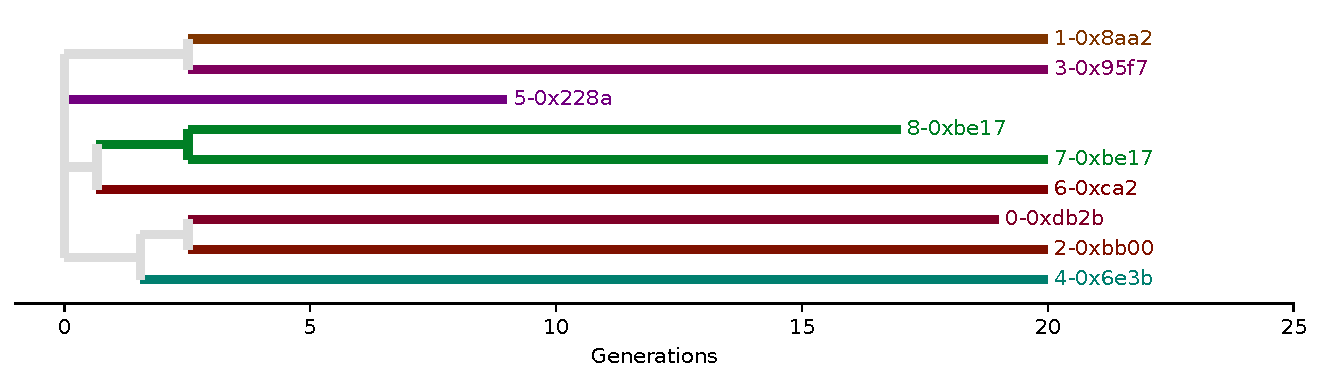
\includegraphics[width=\textwidth]{binder-wse-sketches/binder/teeplots/genome=hsurftiltedsticky_tagged+replicate=debd0010-f2aa-4679-aac6-b7ce94a2482a+viz=draw-biopython-tree+ext=}
    \caption{20 generations}
    \label{fig:tagged_other}
  \end{subfigure}

  \begin{subfigure}[b]{\textwidth}
    \centering
    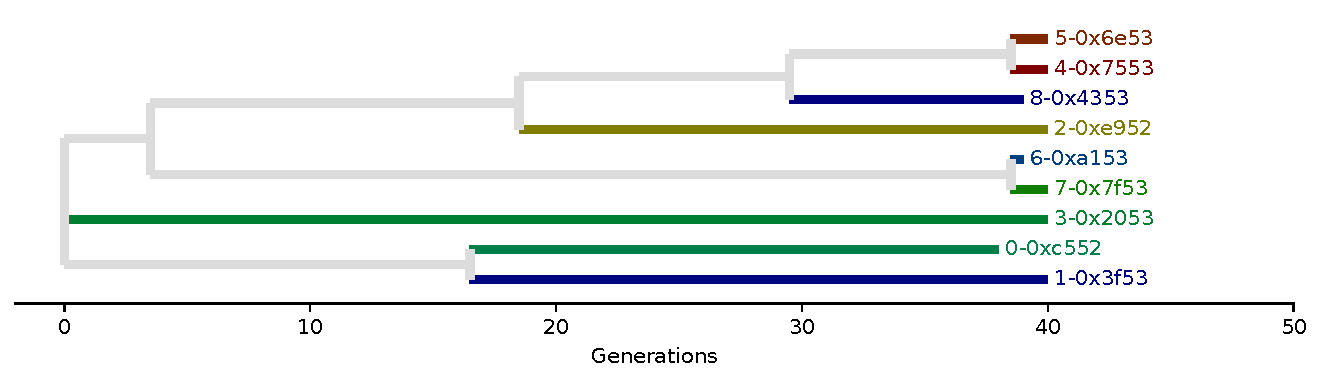
\includegraphics[width=\textwidth]{binder-wse-sketches/binder/teeplots/genome=hsurftiltedsticky_tagged+replicate=14302969-8474-4577-806b-4540da18c605+viz=draw-biopython-tree+ext=}
    \caption{40 generations}
    \label{fig:tagged_other}
  \end{subfigure}

  \begin{subfigure}[b]{\textwidth}
    \centering
    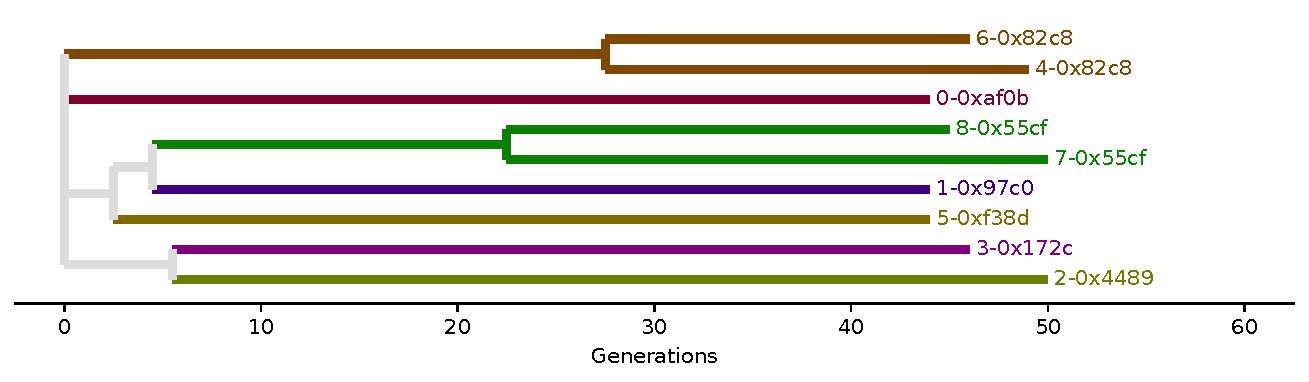
\includegraphics[width=\textwidth]{binder-wse-sketches/binder/teeplots/genome=hsurftiltedsticky_tagged+replicate=c830e722-ad66-48ed-a02f-2aa994dfc268+viz=draw-biopython-tree+ext=}
    \caption{50 generations}
    \label{fig:tagged_other}
  \end{subfigure}

  \begin{subfigure}[b]{\textwidth}
    \centering
    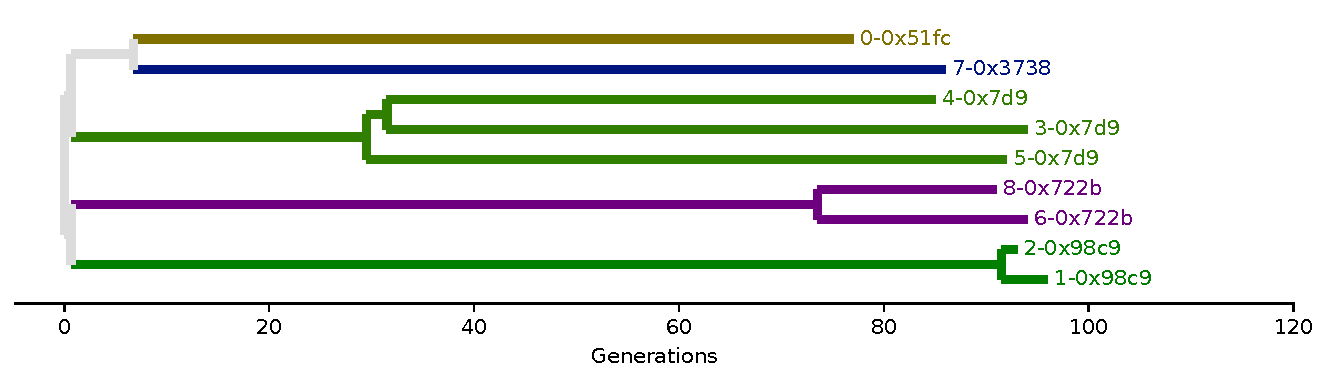
\includegraphics[width=\textwidth]{binder-wse-sketches/binder/teeplots/genome=hsurftiltedsticky_tagged+replicate=a2438095-6857-4a68-bd77-14065953b13c+viz=draw-biopython-tree+ext=}
    \caption{100 generations}
    \label{fig:tagged_other}
  \end{subfigure}
\end{figure*}



% \putbib


% \end{bibunit}

\end{document}
